% Created 2017-07-28 Fri 19:40
% Intended LaTeX compiler: pdflatex
\documentclass[a4paper,12pt]{article}
\usepackage[utf8]{inputenc}
\usepackage[T1]{fontenc}
\usepackage{graphicx}
\usepackage{grffile}
\usepackage{longtable}
\usepackage{wrapfig}
\usepackage{rotating}
\usepackage[normalem]{ulem}
\usepackage{amsmath}
\usepackage{textcomp}
\usepackage{amssymb}
\usepackage{capt-of}
\usepackage{hyperref}
\usepackage[a4paper, total={150mm,237mm}, left=30mm, top=30mm,]{geometry}
\usepackage{fancyhdr}
\pagestyle{fancyplain}
\lfoot{Kevin Nolan - kevinn@tcd.ie}
\rfoot{MMT Thesis proposal 2017}
\author{Kevin Nolan}
\date{\today}
\title{Kevin Nolan MMT thesis 2017}
\hypersetup{
 pdfauthor={Kevin Nolan},
 pdftitle={Kevin Nolan MMT thesis 2017},
 pdfkeywords={},
 pdfsubject={Sketching sounds in the modern web browser},
 pdfcreator={Emacs 25.0.94.2 (Org mode 9.0.9)}, 
 pdflang={English}}
\begin{document}

\maketitle
\setcounter{tocdepth}{4}
\tableofcontents


\section{Introduction}
\label{sec:org5fe1151}
\subsection{Motivations}
\label{sec:org0142afd}
Some primary motivations for the creation of the app are as follows (in no
particular order):
\begin{itemize}
\item Draw attention to concept of more graphically oriented interfaces for
synthesis (UPIC) to a wider audience by presenting the app in a very
accessible format (PWA)
\item Explore the advantages and limitations of prototyping an experimental
interface using web technologies
\item Frustration with the creative flow of commercial DAW applications
\item Over representation of analog type metaphors in both DAW applications and in
the web apps being developed (missed opportunity)
\item Use functional programming techniques such as immutable data structures to
ease the complexity of managing fundamental concerns such as undo.
\end{itemize}

\subsection{Project goals}
\label{sec:org1365b04}
\subsection{Structure of thesis}
\label{sec:org6bf5f0a}

\section{Background}
\label{sec:org5621eb2}

\subsection{DAW analog metaphors}
\label{sec:org46946c1}
One of the primary tools used by electronic musicians today for the production
of music is DAW and it's inherent metaphors based on analog system still reign
supreme in the field \cite{bell_journal_2015}. The familiar concepts of analog
tape machines and mixers benefit the novice user by offering a network of
familiar and tangible real world metaphors in which to carry out their creative
work. However, as well as the benefits that these types of metaphors bring, they
also impose some limitations and bring about certain biases. Musical ideas that
are difficult to realise can be left unexplored.

A particular criticism of the DAW is the difficulty in maintaining and managing
the editing of complex automation information. Automation is the term given to
the continuous altering of aspects of the sound and is usually represented in
lanes separate to the primary note pitch information. It may be recorded in or
drawn in by the producer. Difficulties can arise, when multiple subtly
interacting lines of automation, such as pitch bends and filter changes are
being manipulated. William Coleman gives a particularly clear example of this
and outlines the difficulty of representing "portamento time", the time it takes
a note to slide from one to the next. The visual results can be jarring,
unintuitive and not reflective of the audio results.

\begin{caution}
Duignan (2008) describes a similar problem in his study that monitored
professional producers working in DAW environments
\cite[p. 156]{duignan_computer_2008}. The particular problem identified by
Duignan was that of processing one off effects for single musical events. A
number of convoluted processes were observed, including bouncing the affected
portion to audio, duplicating the track, setting up a particular auxiliary for
the effect and controlling the effect with automation. In these cases, the
hierarchy imposed by the DAW gets in the way, where it could be modeled quite
elegantly in a more open program such as Max Msp. This, unfortunately, raises
the issue of drifting into the area of analytic thinking and away from creative
thinking, a combination that John Cage advises against: "Don't try to create and
analyse at the same time. They're different processes." \cite{popova_10_2012} The
need to explore alternative metaphors is clear. A description of a promising
alternative metaphor, that of drawing/sketching will now be discussed.
\end{caution}

\subsection{Legacy systems}
\label{sec:org909edb2}
\begin{itemize}
\item Oramics
\item UPIC
\end{itemize}

\subsection{Golan Levin etc}
\label{sec:org9ae92ab}


\section{Similar work}
\label{sec:org4c762d3}
\subsection{Criteria}
\label{sec:org47c5792}
\begin{description}
\item[{Web based}] Does the system work on a modern browser
\item[{Symbolic rep}] Does the system use symbolic representation or is it more or
less a spectrum that you can draw on.
\item[{Accessibility}] From none to high, is the system accessible. An example of a
no accessibility is a system like UPIC which is not
accessible to something that is very accessible like web
app. Paid software that needs to be installed is in the
middle of this spectrum.
\end{description}

\begin{center}
\begin{tabular}{llll}
System & Web based & Symbolic rep & Accessibility\\
\hline
SonicPainter & No (although ported by the author) & Yes & Low\\
UPIC & No & Yes & None\\
Oramics & No & Yes & None\\
\end{tabular}
\end{center}

\section{{\bfseries\sffamily TODO} My approach [0/2]}
\label{sec:orgb479b30}
\begin{itemize}
\item $\square$ Come up with a title
\item $\square$ Other stuff
\end{itemize}

\subsection{Adding allowances for stylus}
\label{sec:org8f07cb7}
\subsection{Relationship between control data and synths}
\label{sec:org7a52243}
Discuss Roger Dannenberg conceptualization of the two main paradigms of music
software systems. Resource based vs instance \cite{dannenberg_resource-instance_1991} 
\subsection{Key specifications}
\label{sec:org5cd5246}
\subsection{Paper.js}
\label{sec:orgfdaf4fd}
\subsection{NUI}
\label{sec:orgefb49b6}
Introduce the NUI
\subsection{Tone.js}
\label{sec:org2c4343f}
\cite{mann_interactive_2015}

\section{Execution}
\label{sec:orgce589e3}
\subsection{Early prototypes}
\label{sec:org9eb27cf}
\subsubsection{Melodypainter}
\label{sec:org22be26a}
Thus far, some early test prototypes to establish possible directions for the
application have been built. A Max Msp patch was created which allows the user
to draw freehand lines, which are converted into break point function data and
used as to generate a melodic profile in Bach. This is further processed into a
pentatonic scale. Once input the system plays the resulting melody back. A
notable flaw of the system was that it required users to draw shapes in a
generally horizontal fashion for the data to be of use and to create a strong
relationship between the visuals and the generated music.

\subsubsection{Sonicsketch - shape recognition}
\label{sec:org6d2a166}
A separate application was created in Processing which allowed users to draw
shapes, using either mouse or ideally, pen input and have a sound that is
associated with each shape played back. As the sound of each shape plays back,
it is lit up using animation, creating a strong connection between the shape and
it's resulting sound. The application used the "gesture variation follower"
system \cite{caramiaux_adaptive_2015}, which while promising in principle, didn't
have a high rate of accuracy in recognizing the shapes. It is for this reason
that Microsoft's ink api is now being used for further prototyping.

\subsection{The build out}
\label{sec:org9212529}
\subsubsection{Building the framework}
\label{sec:orgc6f06ed}
\paragraph{Advantages of the react.js model of UI programming}
\label{sec:org0e83cb3}
\subsubsection{Stroke functionality}
\label{sec:org96f80ab}
Describe how the stroke functionality works and was implemented.
\paragraph{Overall app}
\label{sec:org581a076}

\begin{center}
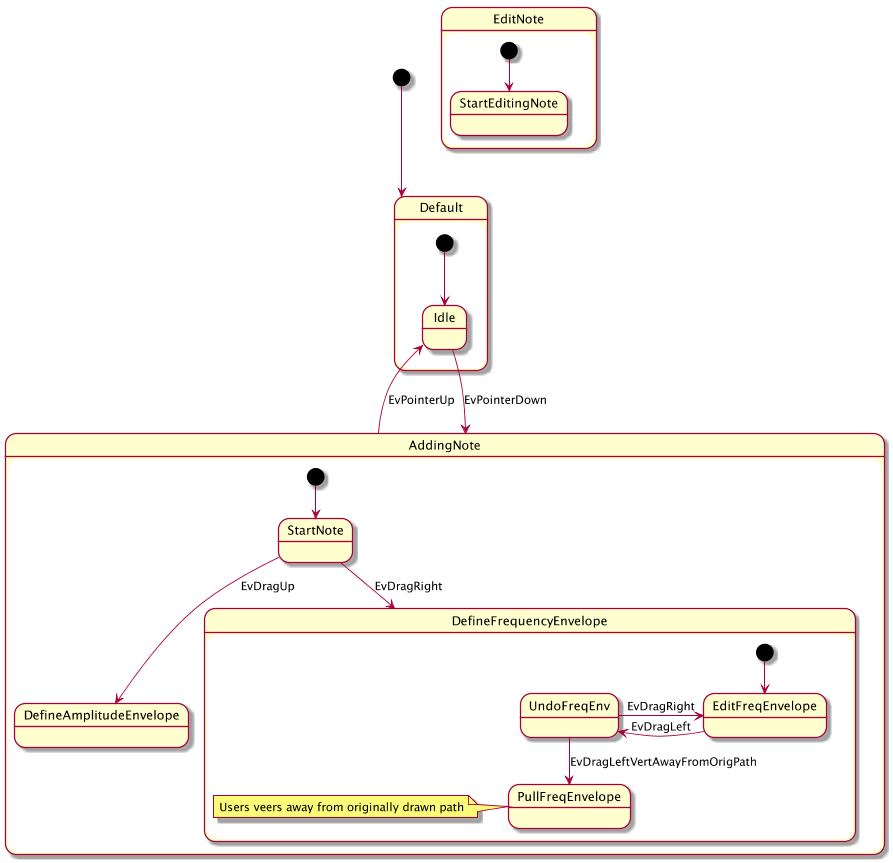
\includegraphics[width=.9\linewidth]{tryout.png}
\end{center}

\begin{enumerate}
\item The relevant code
\label{sec:org25240f3}
\begin{verbatim}
(defn pointer-move [{:keys [temp-obj active-preset]} evt]
  (when-let [{:keys [path group] :as temp-obj} @temp-obj]
    (let [pointer-point (.. evt -point)
          rel-pos       (.. group (globalToLocal pointer-point))]
      (log (.. group -position) "pointer point rel")
      ;; Only add positive points relative to first
      ;; Remove points greater than pointer-points
      (when-let [last-seg (.. path getLastSegment)]
        (log last-seg)
        (let [last-point (-> last-seg .-point)
              pointer-x  (.-x rel-pos)]
          (if (>= pointer-x (.-x last-point))
              (-> path (.add rel-pos))
              (let [greater-segs (filter
                                  #(> (-> % .-point .-x) pointer-x)
                                  (.-segments path))]
                ;; Remove greater points
                (doseq [seg greater-segs]
                  (.removeSegment path (.-index seg))))))))))
\end{verbatim}
\end{enumerate}

\paragraph{Sketch walkthrough}
\label{sec:orgaebcfc6}

\begin{center}
\begin{figure}[htbp]

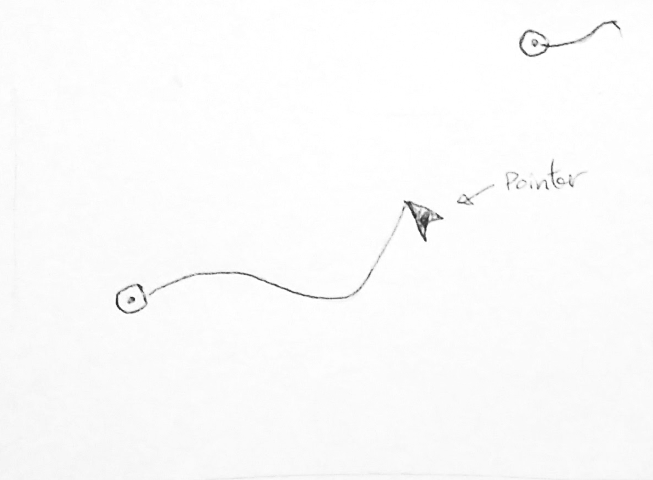
\includegraphics[height=0.2\textwidth]{./charts/images/attractor-01 (Small).png}
\caption{\label{fig:org5f8012d}
This is the caption for the next table (or link)}
\end{figure}


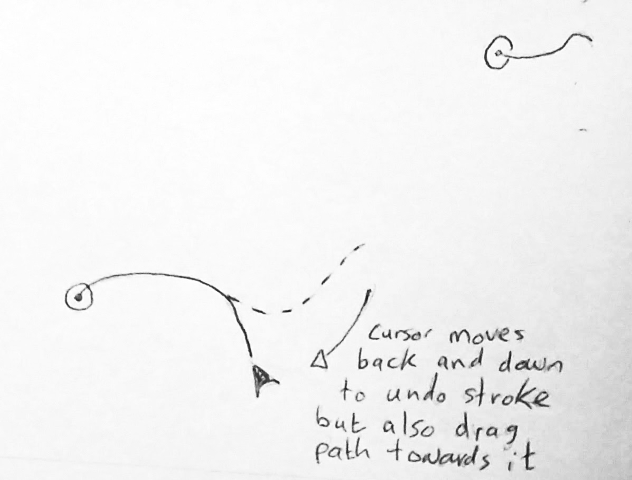
\includegraphics[height=0.2\textwidth]{./charts/images/attractor-02 (Small).png}

\begin{center}
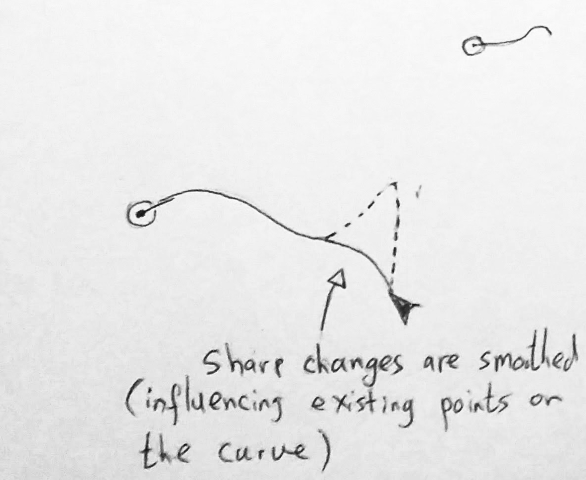
\includegraphics[height=5cm]{./charts/images/attractor-03 (Small).png}
\end{center}
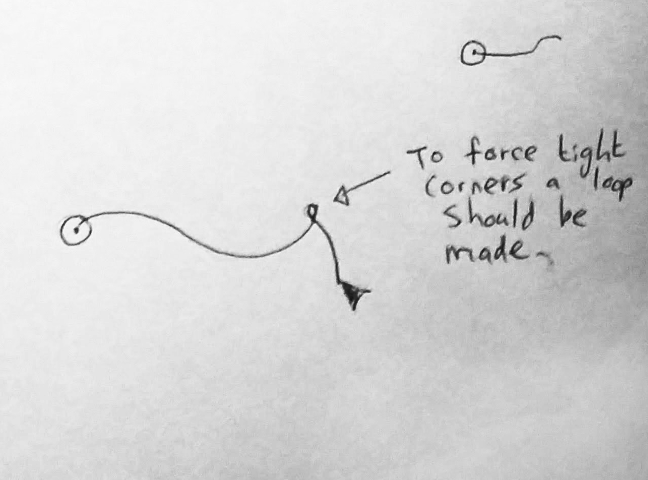
\includegraphics[height=0.2\textwidth]{./charts/images/attractor-04 (Small).png}
\end{center}

Please see [\ref{attractor-01}] 
\subsubsection{Enabling undo and redo}
\label{sec:orgd213a93}
\subsubsection{Catering for additional input types}
\label{sec:orga664014}
Describe issues encountered including a lack of support in paper.js and the
small patch required to enable it.

\section{Evaluation [0/1]}
\label{sec:orgbd01659}
\begin{itemize}
\item $\square$ Come up with a better title.
\end{itemize}

A reasonably functional application was built which allowed for some basic
interactions. While very much a prototype the app does offer the following
innovations:

\begin{itemize}
\item Using the web as a testing ground for new interaction paradigms
\item Using react js and clojurescript to allow for realtime (or close to realtime)
development
\item Delivering a graphical synthesis oriented system in a very accessible format,
a PWA
\item Incorporation of alternative device inputs using the W3C pointer api to allow
for more suitable and accurate input
\item Trial of next generation react framework that extends it's reach beyond html
markup which is the general limit of the original system
\item The result of combining react, clojurescript and tone.js is a declaritive data
DSL to describe audio processing. Potentially very useful as a beginner tool
and as a prototyping tool.
\item Makes the assertion that different tools can be used for different stages of
the creative process and by providing integration into other platforms can be
easily incorporated into the flow.
\item Works as an idea generator. The resulting audio could be sampled and used in
another app
\end{itemize}

Some of the shortcomings of the work:
\begin{itemize}
\item It's very easy to create a mess of frequencies and pitch bends and difficult
or impossible to create standard musical material
\item Suffers from performance issues and can get choked up when too much elements
are added to the screen
\item While some basic and standard useability features have been added such as
undo and redo
\item The sound quality isn't always perfect and some aliasing and other digital
artifacts are in evidence
\end{itemize}


\section{Conclusions and further work}
\label{sec:org3559ffc}
\subsection{Future work}
\label{sec:org3ea7f34}
While SonicSketch in it's current format is useable for further ease of use it
would need work done on performance related issues, including but not limited
to: 
\begin{itemize}
\item Move more processing into web workers
\item Look at compile to wasm based systems instead of Tone.js, including Csound
\item Move graphics to use the GPU more heavily which would mean re-implementing a
good deal of the functionality provided by paper.js
\end{itemize}

Incorporate more dimensions into the visualisation, such as distortion, delay
effects, harmonic structure. Investigate how the visualisations could scale up
to incorporate more information.

Allow for larger structures, perhaps by scrolling.

Allow for meta-strokes where a stroke would draw the contents of another scene.

\section{References}
\label{sec:orgc0a1a79}
\end{document}